\documentclass[11pt]{article} 
\usepackage{graphicx} 
\usepackage[authoryear,round]{natbib} 
\usepackage{caption}  
\usepackage[mathlines]{lineno} 
\usepackage{setspace} 
\usepackage{mathrsfs} 
\usepackage{rotating} 
\usepackage{hyperref}
\usepackage{url} 
\usepackage{amssymb} 
\usepackage{multirow} 
\usepackage[none]{hyphenat} 
\usepackage{verbatim} 
\usepackage{amsmath}
\usepackage{threeparttable}
\DeclareGraphicsExtensions{.pdf,.png,.jpg} 
\setlength{\topmargin}{-.5in} 
\setlength{\textheight}{9in} 
\setlength{\oddsidemargin}{.125in} 
\setlength{\textwidth}{6.25in} 
\doublespacing 


\begin{document}
\begin{linenumbers}
\renewcommand\linenumberfont{\normalfont\small}
\setlength\linenumbersep{1cm}

  \renewcommand{\theequation}{S2-\arabic{equation}}
 
% redefine the command that creates the equation no. 
\setcounter{equation}{0}  % reset counter 
\section*{Supplementary Information S2 - Model details for simulation of evolving neonate mass in the face of ontogenetic niche shifts}

In many species, the ability of individuals to exploit different resources changes as individuals grow in size or develop across life stages, a process referred to as an ontogenetic niche shift (\citealt{werner84}). When consumption by conspecifics causes resource limitation, ontogenetic niche shifts can impose distinct patterns of density-dependence during an individual's life cycle. Such density-dependence could affect the ability of newborns to survive, grow and mature, potentially affecting patterns of life history evolution (e.g., \citealt{mueller91}). For instance, evolutionary changes in neonate mass are subject to a trade-off between selection for larger clutch sizes and increased offspring survivorship (e.g. \citealt{lack66}, \citealt{parker86} and \citealt{roff01}). However, the strength of this trade-off itself can depend upon prevailing patterns of resources available for juvenile growth (necessary for escaping vulnerable size classes) and adult reproduction (which partially governs the number of offspring a parent can birth or sire). These patterns of resource availability at different life stages may, in turn, depend on the strength of an ontogenetic niche shift individuals experience.

To understand the effect of ontogenetic niche shifts on the evolution of neonate mass, we use sPEGG to model a physiologically-structured (e.g., \citealt{persson98} and \citealt{deroos01}), sexually reproducing consumer population whose individuals utilize and compete over two dynamic, biological resources. We assume maximum resource consumption rates increase allometrically (\citealt{brown04}), but that individuals transition from utilizing one resource type to utilizing another as they increase in size. We model offspring size at birth as an evolvable trait controlled additively by a finite number of loci of large effect. We assume survivorship increases monotonically with individual size (e.g., \citealt{werner84}), but that parents with larger neonates also birth fewer offspring (e.g., \citealt{parker86}). 

\subsection*{Model overview}
We consider a size-structured, sexually reproducing consumer population. Our model has two key components - an ecological component and a genetic component. The ecological component describes the individual's interactions with their environment. We model how differential reproductive success and survivorship (fitness) among individuals emerge from these diverse interactions. The genetic component specifies the genetic distribution for neonate mass, and how the genetic distribution changes between generations. 

The model's dynamics are iterated on a discrete time step. At each time step, the model cycles through all individuals to determine their fates. We assume that the organisms reproduce once every $T$ time-steps; thus, each time-step can be thought of, for instance, as a day for a specie's with an annual breeding season. Our model applies to organisms with overlapping generations and seasonal reproduction such as insects, marine invertebrates, and vertebrates that live in seasonal environments. We also partition individual somatic mass $W$ into reversible ($Y$) and irreversible ($X$) mass to explicitly study how energetic constraints affect individual reproductive decisions. 

The model's parameters characterize the selective pressures and the genetic, energetic and ecological constraints on the population. Its ecological dynamics are driven by four key processes: resource consumption, somatic growth, mating, and mortality. Below, we describe how each process is modelled in further detail. Table S2-1 provides a summary of the model's ecological components. 

\subsection*{Resource Consumption}
We consider two dynamic, biological resources which the consumers utilize and for which they compete. Resource availability can regulate individual somatic growth, and ultimately affects individual survivorship and reproduction. Thus, considering two resources allows us to model situations where newborns and large adults potentially experience different regulation regimes, and hence permit different forms of resource scarcity to operate during an individual's lifetime. 

The instantaneous resource-consumption rate $E_{i,{\tau},j}$ of individual $i$ of resource $j = 1,2$ at time $\tau$ is a function of its body size (somatic mass $W_{i,\tau}$) and resource density $R_{\tau,j}$:
\begin{linenomath}
\begin{equation}
E_{i,\tau} (R_{\tau,j}, K_j, W_{i,\tau}) =  h(R_{\tau,j},K_j) \pi(W_{i,\tau}, j) \alpha W_{i,\tau}^{\gamma} 
\end{equation}
\end{linenomath}
where $\pi(W_{i,\tau}, j)$ describes the proportion of a individual $i$'s diet that consist of resource type $j$, and $h(R_{\tau,j}, K_j)$ describes the proportion by which an individual's resource consumption decreases when the resource density $R_{\tau,j}$ falls short of the maximum daily consumption rate (attained when the resource density is at carrying capacity $K_j$). 

We assume that if the resources are at their carrying capacities, then an individual's instantaneous resource consumption rate depends allometrically on its body size, where the parameters $\gamma$ and $\alpha$ are an allometric exponent and an allometric constant scaling consumption rates, respectively (e.g., \citealt{west01}). 

The size-independent function $h(R_{\tau,j},K_j)$ describes how much an individual's consumption of resource $j$ decreases as the becomes more scarce. For example, if resource $j$ has carrying capacity $K_j$ and consumer individuals display a Holling type-II functional response with attack rate $a$ and handling time $T_H$, then $h(R_{\tau,j},K_j)$ describes how resource limitation constrains consumption, i.e., $h(R_{\tau,j},K_j) =\frac{a R_{\tau,j}/K_j}{1 + a T_H R_{\tau,j}/K_j}$. 

We assume that the amount of a given resource of type $j$ a consumer utilizes depends on the consumer's size. Such ontogenetic niche shifts are common in nature (e.g., \citealt{werner84}). For example, many fish are planktivorous when small, but shift to piscivory as they increase in size (e.g., \citealt{claessen02}). The function $\pi(X_{i,\tau}, j)$ describes the proportion of individual $i$'s diet that consist of resource type $j$. The function $\pi(X_{i,\tau},j)$ is modeled to depend on both anatomical structures such as gape-size and body length that contribute to irreversible mass  (e.g., \citealt{werner84}). It is also determined by a constant $u$ that governs what fraction of the adult resource base very small individuals consume, and the steepness $p$ of the curve as individuals grow. Thus, $\pi(X_{i,\tau},j)$ is defined by the following logistic equations:

\begin{linenomath}
\begin{equation}
\label{eqn:pi}
\pi(W_{i, \tau}, j) = \left\{ \begin{array}{ll}
\frac{1}{1 + \exp(- p(W_{\tau,i} - u W_{max}))}, & \textrm{if } j = 1 \\
1 - \frac{1}{1 + \exp(- p(W_{\tau,i} - u W_{max}))}, & \textrm{if } j = 2 
\end{array} \right.
\end{equation}
\end{linenomath}

l[] is a function mapping irreversible mass to body length(e.g., \citealt{agresti02} and \citealt{claessen02}). We highlight that when $\pi(X_{i, \tau}, j)$ is invariant with $X_{i,\tau}$ (e.g., $p$ small), this describes a situation where resource scarcity affects all individuals similarly during their life-time.

Resource variability is driven by both extrinsic and intrinsic sources of variability. Extrinsic sources of variability, such as climactic fluctuations, affect the per-capita intrinsic growth rate $r_j^{\prime}$ of resource $j$. By contrast, temporal variation in resource utilization by the consumer generates variability in resource levels that is intrinsic to the system.

We assume that the dynamics of resource $j$ are described by intrinsic, density-dependent growth and predation by the consumer (e.g., \citealt{claessen00}) and are governed by the following Beverton-Holt-like growth curve:
\begin{linenomath}
\begin{equation}
R_{\tau+1,j} = \frac{r_j^{\prime} R_{\tau,j}}{1+(R_{\tau,j})/K_j}  - \sum_{i=1}^{N_{\tau}} E_{i,\tau,j} (R_{\tau,j})
\end{equation}
\end{linenomath}
where $E_{i,0,j} (R_{0,j})$ is the consumption rate of resource $j$ by the individual consumer $i$ at the start of the time step, and $N_{\tau}$ is the population size of consumers at the beginning of the time step. 

We model stochastic fluctuations in the resource dynamics due to extrinsic factors, such as climactic variability, by allowing $r_j^{\prime}$ to vary from time step to time step by drawing the actual value of $r_j^{\prime}$ used in the evaluation of $R_{t,j}^{\star}$ from a normal distribution with mean $r_j$ and standard deviation $e_{r,j}$. Our model does not consider externally imposed deterministic fluctuations. Hence, temporal variability in resource abundance and the consumer's population dynamics are emergent properties of the underlying ecological processes we model, as well as the stochastic nature of the model itself. 

\subsection*{Somatic Growth}
In our model, somatic growth generates size structure. We model two components of somatic growth: growth in irreversible mass $X$ and growth in reversible mass $Y$. An individual's irreversible, or structural, mass $X$ consists of compounds such as organ and skeletal tissue that cannot be starved away (e.g, \citealt{broekhuizen94} and \citealt{deroos01}). Irreversible mass can be viewed as a surrogate for body length, which does not decrease even under starvation conditions (e.g., \citealt{broekhuizen94}). By contrast, an individual's reversible mass is determined by energy reserves such as lipids and gonadal tissue in mature individuals that can be starved away. Reversible mass is partitioned into the mass of storage tissue $Y$, and, in mature individuals, the mass of gonadal tissue, $G$ (e.g., \citealt{broekhuizen94}, \citealt{persson98}, \citealt{deroos01}) (Fig. 1B). Hence,
\begin{linenomath}
\begin{equation}
W = X + Y + G.
\end{equation}
\end{linenomath}
In females, gonadal mass $G$ consists largely of reproductive tissue, while in males, gonadal mass $G$ is interpreted as the amount of reversible mass allocated to reproduction through the loss of somatic mass incurred by competing with other males for access to mature females as well as the production of reproductive tissue.

We assume that individuals are born with the maximum reversible mass to irreversible mass ratio. We define an individual's condition, $c$, as the ratio of storage tissue mass to total somatic mass, i.e., $c=\frac{Y}{W}$. 

An individual consumer's size at maturity and the fraction of resources it allocates towards reproduction affects how it allocates its energetic intake between irreversible, reversible, and gonadal mass. Here, we seek to link resource consumption to an individual's physiological state mechanistically. An individual's physiological state (e.g., body size, condition, etc...) determines its performance (in particular, survivorship and reproduction). Therefore, explicating how metabolic constraints affect somatic growth is key to describing the feedback between an individual's environment and its physiological state.

A consumer with mass $W_{i,\tau}$ at time $\tau$ grows according to the following growth equation (e.g., \citealt{west01})
\begin{linenomath}
\begin{equation}
\label{eqn:growth1}
W_{i,\tau+1} = H(R_{\tau}, W_{i,\tau}) \alpha W_{i,\tau}^{\gamma}  - \delta W_{i,\tau},
\end{equation}
\end{linenomath}
where $\delta$ describes the metabolic rate per unit mass of consumer tissue, $H(R_{\tau}, W_{i,\tau}) = \sum_{i=1,2} (h(R_{\tau,j}, K_j) \pi(W_{i,\tau}))$ describes how resource scarcity ($R_{\tau}$) at time $\tau$ reduces the growth rate of an individual of size $W_{i,\tau}$, and the parameters $\gamma$ and $\alpha$ are an allometric constant and an allometric exponent scaling consumption. We therefore assume that when the mass derived from consumption exceeds metabolic costs, any surplus mass is invested in somatic growth. For taxa with indeterminate growth, $W_{max}$ represents an asymptotic body size which individuals approach at a decelerating rate. For taxa with determinate growth, $W_{max}$ simlpy defines the body size at which the somatic growth rate is zero. We assume $\gamma \leq 1 $ so that there is an asymptotic maximum size $W_{max}$ beyond which matabolic costs render further somatic growth impossible (for empirical values of $\gamma$, see, e.g., \citealt{moses08}).

Consumer individuals are assumed to be born with the maximum ratio $q_J$ between reversible mass and irreversible mass. We note that at birth, an individual's reversible mass does not include gonadal mass - instead, reversible mass consists of storage tissue such as fats. Upon maturation, reversible mass includes the mass of gonadal tissue as well as storage tissue. Hence, the corresponding maximum ratio between reversible mass and irreversible mass for adults is given by $q_A > q_J$. Because reversible mass can be starved away, it represents a reserve that individuals can utilize during periods of resource limitation. Thus, when resources are not limiting, we assume consumer individuals will maintain the maximum ratio of reversible to irreversible mass. The fraction $\kappa$ of $ \Delta W_i = W_{i,\tau+1} - W_{i,\tau}$ that is allocated to irreversible mass depends on the ratio of reversible to irreversible mass; thus:
\begin{linenomath}
\begin{equation}
\label{eqn:growth1}
X_{i,\tau+1} = \kappa \frac{Y_{i,\tau}}{X_{i,\tau}} \Delta W_i + X_{i,\tau+1},
Y_{i,\tau+1} = (1-\kappa \frac{Y_{i,\tau}}{X_{i,\tau}}) \Delta W_i + Y_{i,\tau+1}.
\end{equation}
\end{linenomath}

Hence, $\kappa$ describes a constraint on how much an individual can allocate resource intake towards fending off starvation risk (by improving condition) instead of reducing other forms of density-independent mortality by increasing irreversible mass.

In mature individuals, a fixed proportion $\rho_i$ of $1-\kappa \frac{Y_{i,\tau}}{X_{i,\tau}}) \Delta W_i$ is set aside for reproduction. For example, in female animals this takes the form of allocation to reproductive tissue mass $G_i$, while in males this represents, for example, the mass loss associated with searching and securing female mates as well as the energy expended in producing gonadal tissue. For simplicity, we assume the mass of reproductive tissue in juveniles is negligible. Thus, at the end of each time step, reproductive tissue mass for individual $i$ is given by:
\begin{linenomath}
\begin{eqnarray}
\label{eqn:allocations}
G_{i,\tau+1} &=& I_f \times (Y_{i,\tau} - X_{i,\tau} q_A)
\end{eqnarray}
\end{linenomath}
where $I_f = 0$ if the individual is immature, $I_f = 1$ if the individual is mature. The growth equations above are based on the assumption that all reproductive tissue mass from the previous time step was spent on reproduction during that time step. Following reproduction, the gonadal mass $G_{i,\tau+1}$ is deducted from the individual's reversible mass $Y_{i,\tau}$.

Equations (\ref{eqn:allocations}) summarize how energetic constraints govern the feedback between an individual's environment and its physiological state. In particular, they describe how resource use affects an individual's reproductive success (which depends on gonadal mass $G$) and survivorship (which depends on irreversible mass $X$ and condition $c=Y/(X+Y+G)$).

\subsection*{Reproduction}
Individual consumers breed once every $T$ time steps, and we assume random mating between males and females, conditioned on gonadal mass. If, prior to mating, an individual consumer $i$'s irreversible mass $X_i$ is larger than its size at maturity ($\sigma_i$), then individual $i$ is considered to be mature. 

The number $F$ of fertilized eggs in the population is determined by three variables: (1) the average neonate mass of offspring of female $i$, $\Omega_i + q_J \Omega_i$, where $q_J$ is the maximum ratio of reversible mass to irreversible mass, (2) the reproductive tissue mass of female $i$ $G_i$, and (3) $N_{f,t}$, the total number of mature females in time step $t$. Then,
\begin{linenomath}
\begin{equation}
\label{eqn:fecundity}
F = \sum_{i=1}^{N_{f,t}} \frac{G_i}{\Omega_i + q_J \Omega_i}
\end{equation}
\end{linenomath}
The present modeling framework applies to both viviparous and oviparous organisms. However, for simplicity, we discuss model development in terms of an oviparous organism. 

For each egg, the mother and father are drawn at random from mature males and females in the population. The probability that the egg comes from female $i$ is a function of the female's relative gonadal mass $G_i$ in the population,
\begin{linenomath}
\begin{equation}
\label{eqn:Femalerepr}
\Pr(\textrm{female $i$ produces an egg} | G_i) = (\frac{\frac{G_i}{\Omega_i + q_J \Omega_i }}{F})^{v_f},
\end{equation}
\end{linenomath}
where $v_f$ describes the severity fo reproductive skew among females.

\indent Similarly, the probability that a mature male $i$ fertilizes a given egg is a function of its irreversible mass, $X_i$, relative to the mass of other mature males in the population. In particular, our model reflects the common observation that body size (often measured as length, which depends on irreversible mass) is positively correlated with reproductive success in males (e.g., \citealt{trivers72}, \citealt{blanckenhorn05}), and a male's relative structural mass is incorporated into calculating the probability of fertilization as: 
\begin{linenomath}
\begin{equation}
\Pr(\textrm{male $i$ fertilizes an egg} |X_i, G_i) = \frac{X_i^{v_m}}{\sum_{j=1}^{N_{m,t}}(X_j)^{v_m}}
\end{equation}
\end{linenomath}
where $N_{m,t}$ is the total number of mature males, and $v_m$ determines how strongly a male's reproductive value increases with its relative irreversible mass. The parameter $v_m$ can describe a host of biological processes, including female preference for larger males and the superior fighting ability of larger males. High values of $v_m$ characterize populations where reproductive success is strongly correlated with male body size, while lower values of $v_m$ characterize populations where male reproductive success is similar across a range of body sizes. 

\subsection*{Mortality}
\indent At any given time step, the number $\Phi$ of newborns that survive to the juvenile stage depends on the population's total egg production (e.g., \citealt{wootton98}). Several mechanisms can contribute to such density-dependent mortality at the earliest life stages (\citealt{shepherd80}). For instance, in many organisms early life stages (e.g., larvae) are particularly vulnerable to predators that can be attracted to large aggregations of eggs or hatchlings (\citealt{martin93}, \citealt{bellinato95}, and \citealt{white07}). Furthermore, when hatchlings or early larvae form dense aggregations over small spatial scales, such aggregations can lead to the rapid exhaustion of locally available resources (e.g., \citealt{leggett94}, \citealt{arino98}). Finally, in many organisms,  dispersal occurs at very early stages of the life cycle. In such situations, the ability of newborns to become established and survive to maturation at suitable sites depends, in part, on the fraction of sites already occupied by breeding adults, which in turn affects the value of $F$ (eq. (\ref{eqn:fecundity}) e.g., \citealt{caley96}). For example, in several coral reef fishes, the density of adults is inversely correlated with the survivorship of juveniles, possibly because of competition faced by juveniles for suitable shelter sites that protect individuals from predation or the availability of desirable feeding sites (e.g., \citealt{sale76}, \citealt{forrester95}, \citealt{caley96}, and \citealt{wilson02}). When these mechanisms interact, as when limited resource availability stunts somatic growth and thereby keeps new borns from growing out of vulnerable size classes, the relationship between the number of surviving newborns and total fecundity is described by classical stock-recruitment curves (\citealt{shepherd80}).

Here we model the density-dependent recruitment $\Phi$ according to the function:
\begin{linenomath}
\begin{equation}
\Phi = \frac{\nu}{1+N_f},
\end{equation}
\end{linenomath}
where $\nu$ is a constant and $N_f$ is the total number of reproductive females. For viviparous organisms, $\Phi$ can be interpreted as the fraction of offspring that survive past a weaning period. 

\indent In addition to density-dependent mortality of newborns, individual survivorship from one time step to the next is a function of the individual's irreversible mass. We assume that the probability that an individual survives from one time step to the next is described as
\begin{linenomath}
\begin{eqnarray}
\label{eqn:survivorship1}
\Pr(\textrm{individual $i$ survives} | X_{i,t}) = \frac{1}{1+\exp(-\beta_2 (X_{i,t} - \beta_1))}
\end{eqnarray}
\end{linenomath}
This functional form results from using standard logistic regression to model survivorship probability as a function of size, as is frequently recommended (e.g., \citealt{morris02}, \citealt{ellner06}, and \citealt{hesse08}). The parameter $\beta_1$ represents the mass (scaled by the maximum irreversible mass $W_{max}$) at which the mortality risk is equal to 1/2. The parameter $\beta_2$ characterizes the steepness of the survivorship curve around this point. This functional form is quite flexible, and depending on the values of $\beta_1$ and $\beta_2$ can describe an exponential increase in survival with increased irreversible mass, a sigmoidal increase in survival with larger irreversible mass, a relatively linear increase in mortality risk with irreversible mass, or a rate of mortality that is largely independent of body size.

We further assume that individuals also suffer an additional source of mortality due to starvation. We assume that as individual condition worsens, starvation risk increases and survival decreases at an exponential rate. The survivorship function thus depends on individual condition and somatic mass as:
\begin{linenomath}
\begin{eqnarray}
\label{eqn:survivorship}
  \Pr(\textrm{individual $i$ survives at time $t$} | X_{i,t},c_{i,t}) = (1-\exp(-\beta_s Y_{i,t}/X_{i,t})) \times \frac{1}{1+\exp(-\beta_2 (X_{i,t} - \beta_1))}. 
\end{eqnarray}
\end{linenomath}
The parameter $\beta_s$ characterizes how survivorship increases exponentially with improving condition. Because resource availability governs somatic growth rates and determines an individual's body size and condition, eq. (17) accounts for the potential for density-dependent processes to affect survivorship throughout an individual's life cycle.

Size-specific mortality links an individual's physiological state to its performance. Size-specific mortality can directly select for different neonate sizes, as well as generate population fluctuations and induce variability in resource availability (e.g.,  \citealt{stearns76}, \citealt{costantino97}, \citealt{deRoos031} and \citealt{ernande04}). In turn, these patterns of temporal variability could subsequently affect the evolution of life history syndromes (e.g., \citealt{winemiller92}).


\subsection*{Genetics}
In our model, the fitness of individuals emerges from their interactions with other individuals and their environment. The evolutionary response of the population to selection on individuals depends on the genetic distribution among individuals. Moreover, the genetic distribution, in turn, is determined by the combined effects of mutation, recombination, and selection. In individual-based models, describing the population's genetic distribution requires we specify the distribution of genotypes among individuals. Thus, specifying how multiple life history traits evolve requires explicit consideration of the genetics underlying the life history traits. Below, we describe how we model the genetics and transmission of the life history traits.

We analyze evolution in the mean irreversible mass $\Omega$ of offspring at birth (neonate mass). While survivorship often increases monotonically with individual size (e.g., \citealt{werner84}), parents that give birth to larger neonates give birth to fewer offspring (e.g., \citealt{parker86}). Thus, focusing on neonate mass allows us to study a trait that directly evolves in response to a trade-off between clutch size and offspring survivorship (e.g. \citealt{lack66} and \citealt{roff01}). 

We assume that offspring size at birth $\Omega$ is a quantitative traits whose genetic values are additively determined by $N_\Omega$ trait-specific loci. The genome is diploid, individuals reproduce sexually, and there is free recombination between all loci. Pleiotropy is absent from the model, and the allelic values of the loci vary continuously over the biologically feasible range of the life history trait. To describe the evolution of this life history trait, we track the dynamics of the alleles and loci underlying the trait explicitly. Such an explicit, multi-locus framework allows us to characterize and account for changes in the genetic distribution of the trait over time. All loci were treated as autosomal and freely recombining with other loci. The allelic values of the loci could change by mutations and the effect of mutations on the allelic values are assumed to be Gaussian distributed. We note that when the number of trait-specific loci approaches infinity and individual allelic effects decline to zero, these assumptions allow our model to recover the classical infinitesimal model used in quantitative genetics (e.g., \citealt{bulmer85b}). 

Prior to reproduction, each parent produces haploid gametes consisting of half the parent's alleles (e.g., \citealt{van06}). Mutations occur with a probability $\mu$ at each locus. If a mutation occurs at a locus, the new allelic value is drawn from a normal distribution with the mean at the allelic value prior to mutation and a standard deviation given by $\varpi \times$ the mean initial allelic value. The gametes from both parents fuse to produce an offspring's diploid genome. The offspring's genetic value at each locus is given by the midpoint of the parental gamete's allelic values at that locus. Thus, the offspring's genetic value for $\Omega$ is the sum of the genetic values across all $N_\Omega$ loci. 

Once an individual's genotypic value is additively determined, its phenotypic value is determined first by drawing a random variable, $z_J$ from a normal distribution with the mean given by the genotypic value and a trait-specific standard deviation $\varrho_J$. In effect, determining the phenotypic value in this way is analogous to specifying the residual variance for the trait (i.e., the difference between the trait's phenotypic and additive genetic variances - e.g., \citealt{houle96}). Thus, if $A_{i,f}, A_{i,m}$ denote the allelic value at locus $i$ an individual inherited from its female and male parent, respectively, and $N(M,\varrho)$ describes a normal distribution with mean $M$ and standard deviation $\varrho$, the individual's phenotypic value $z_J$ is a random variable given as:
\begin{linenomath}
\begin{eqnarray}
\label{eqn:phenval}
z_J \sim N(\displaystyle\sum_{i=1}^{N_J} \frac{1}{2} (A_{i,f} + A_{i,m}), \varrho_J).
\end{eqnarray}
\end{linenomath}

Life history traits appear to generally have low heritabilities (e.g., \citealt{mousseau87} and \citealt{price91}). Nevertheless, there is some question about the relative importance of dominant and epistatic effects among loci for life history traits (e.g., \citealt{roff06}) or whether environmental, gene-by-environment interactions, and developmental processes account for the low heritability in life history traits (e.g, \citealt{price91}, \citealt{houle96}, \citealt{burger00}). Because $\varrho_J$ is shared across individuals, our model formulation effectively assumes most of the residual variance reflects the effects of developmental and (unspecified) environmental effects rather than nonadditive genetic components. 

Finally, the values of $z_J$ were transformed using standard approaches to ensure the expressed phenotypic values were biologically realistic. In particular, we set  
\begin{linenomath}
\begin{eqnarray}
\label{eqn:survivorship}
z_J^{\prime} = \exp(z_J),
\end{eqnarray}
\end{linenomath}
for neonate mass at birth. Thus, when the genetic values of these traits follow a normal distribution, the genetic component of their phenotypic values follow a lognormal distribution (e.g., \citealt{lynch97}).


\subsection*{Analysis and Results}
We vary the density-independent, per-capita recruitment rate of the resource consumed by smaller individuals to assess how shifting the relative availability of juvenile and adult resources affects the evolution of offspring size at birth.  The parameter values used in the simulations of this model employed in the main text are available at \nolinkurl{https://github.com/kewok/spegg}. We find that depending on the relative availability of these resources, the consumer population can evolve towards two potential evolutionary endpoints. The first endpoint occurs where individuals give birth to a large number of small offspring. The second endpoint occurs where individuals give birth to a small number of large offspring (Supplementary Fig. S2). If the juvenile resource is relatively scarce, then this selects against parents that give birth to small offspring, who can remain in vulnerable size-categories until they acquire sufficient resources for growth. By contrast, if the juvenile resource is more abundant, this permits relatively rapid juvenile growth even by small offspring. This relaxes the offspring survivorship-clutch size trade-off, favoring the evolution of smaller body sizes at birth. The model illustrates how differences in a phenotype of the resource species (in this case, per-capita density-independent recruitment) can cascade through ontogenetic changes in the consumer to select for distinct consumer life-history strategies.

\end{linenumbers}

\bibliographystyle{cbe}	
\bibliography{myrefs}

\newpage
\begin{singlespace}
\begin{table}
\begin{center}
\begin{tabular}{l lp{3cm}}
\hline 
\multicolumn{2}{c} {Definition of State Variables and Individual-level Functions} \\ 
\hline
 $W_{i,t} \doteq$ Somatic mass of consumer individual $i$, which is the sum of irreversible (e.g., skeletal & \\
 \hspace{1cm} and muscle tissue) mass, $X_{i,t}$, and reversible mass (storage tissue, $Y_{i,t}$, and & \\
\hspace{1cm} mass of reproductive tissue (for mature individuals), $G_{i,t}$) at time $t$ & \\
 $F_t \doteq$ The number of fertilized eggs in time step $t$ &\\
 $N_{j,t} \doteq$ The number of mature individuals of sex $j$ in time-step $t$ &\\
 $\Omega_i \doteq$ The average irreversible mass of consumer individual $i$'s offspring &\\
 $\Phi_t \doteq$ The number of offspring surviving past the reproductive season in time-step $t$ &\\
 $R_{\tau,j} \doteq$ The biomass of resource $j$ at time $\tau$ &\\
 $N_{t} \doteq$ The number of consumers at time-step $t$&\\
 $E_{i,\tau} (R_{\tau,j}) \doteq$ The amount of resource $j$ consumed by consumer $i$ at time $\tau$ &\\
 $h(R_{\tau,j},K_j) \doteq $ Analogous to the functional response; describes the proportion by which consumer & \\ \hspace{1cm}individual $i$'s consumption of resource type $j$ is reduced by resource scracity. & \\
 $H(R_{\tau}, W_{i,\tau}) \doteq $ The effect of resource scarcity on consumer growth. \\
\hline
\multicolumn{2}{c} {Model Specification: Individual Level Processes}  \\ \hline
 Maturity condition for consumer $i$: $I_f = 1\textrm{ if }X_{i,t} \geq \sigma_i$, 0 otherwise & \\
 $\Pr(\textrm{mature female $i$ is mother of an egg} | G_i) = \frac{\frac{G_{i,t}}{\Omega_i + q_J \Omega_i }}{F_t}$ & \\
 $\Pr(\textrm{mature male \textit{i} fertilizes an egg} |X_i, G_i) = \frac{(X_{i,t})^{v_m}}{\sum_{j=1}^{N_{m,t}}(X_{j,t} )^{v_m}}$  & \\
 $\Pr(\textrm{individual \textit{i} survives between \textit{t}, \textit{t}+1} | X_{i,t},Y_{i,t}) = (1-\exp(-\beta_s Y_{i,t}/X_{i,t})) \times \frac{1}{1+\exp(-\beta_2 (X_{i,t} - \beta_1))}$  & \\
 $\frac{E_{i,\tau}(R_{\tau,j})}{\sum_{k=1}^{2} E_{i,\tau}(R_{\tau,k})} =\pi(W_{i, \tau}, j) = \left\{ \begin{array}{ll}
\frac{1}{1 + \exp(- p (W_{\tau,i} - u W_{max}))}, & \textrm{if } j = 1 \\
1 - \frac{1}{1 + \exp(- p (W_{\tau,i} - u W_{max}))}, & \textrm{if } j = 2 
\end{array} \right. $ \\

 $E_{i,\tau} (R_{\tau,j}) =  h(R_{\tau,j},K_j) \pi(W_{i,\tau}, j) \alpha W_{i,\tau}^{\gamma}$  & \\ 
$W_{i,t+1} =  H(R_{\tau}, W_{i,\tau}) \alpha W_{i,\tau}^{\gamma}  - \delta W_{i,\tau}$\\
$\Delta W_i = W_{i,t+1} - W_{i,t}$\\
$X_{i,\tau+1} = \kappa \frac{Y_{i,\tau}}{X_{i,\tau}} \Delta W_i + X_{i,\tau+1}$ & \\
$Y_{i,\tau+1} = (1-\kappa \frac{Y_{i,\tau}}{X_{i,\tau}}) \Delta W_i + Y_{i,\tau+1}$ \\
$G_{i,t+1} = I_f \times (Y_{i,\tau} - X_{i,\tau} q_A)$ &  \\
\hline
\multicolumn{2}{c} {Model Specification: Population Level Processes} \\ \hline
  $F_t = \sum_{i=1}^{N_{f,t}} \frac{G_{i,t}}{\Omega_i + q_J \Omega_i }$ & \\
  $\Phi_t = \frac{\kappa_1 F_t}{1 + (\frac{F_t}{\kappa_2}^{\kappa_{3}})}$ & \\
 $N_{t} = \Phi_t +N_{t-1} -$ Individuals that  die between ($t-1$) and $t$ \\ 
\hline
\end{tabular}
\caption*{Table S-2: Definition of the state variables in the ecological component of the model and a summary of the model's dynamics. The text provides justifications of the functional forms and a detailed formulation of the model. See text for the definitions of the parameters.}
\end{center}
\end{table}
\end{singlespace}

\newpage
\begin{figure}[h!]
   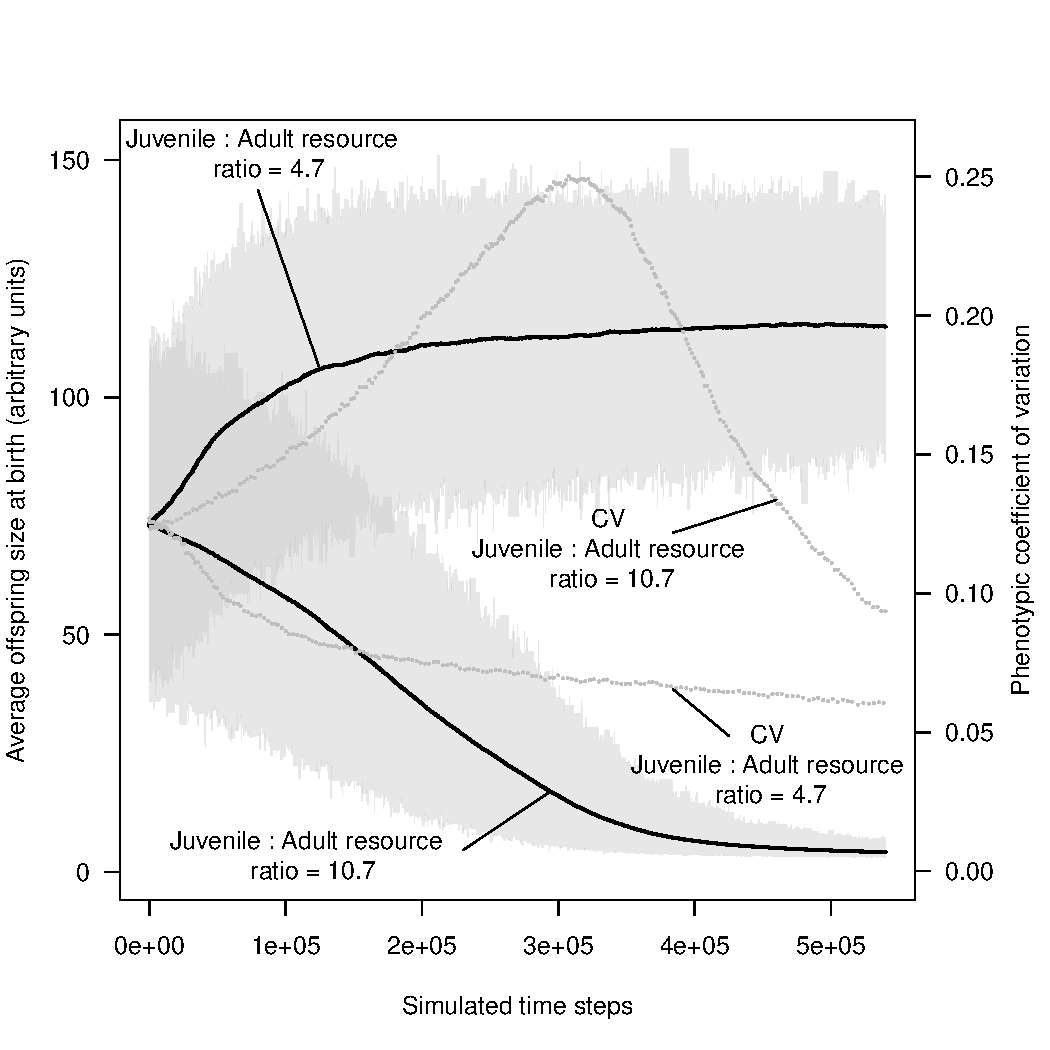
\includegraphics[width=\linewidth] {SupplementaryFigures/FigS2.pdf}
\end{figure}
Supplementary Figure S2. The effect of relative resource scarcity of the juvenile resource on the evolution of body size of an individual at birth. Depending on how scarce juvenile resources are, alternative evolutionary trajectories in average body size at birth (black lines) and the phenotypic variance (illustrated here with the coefficient of variation) for neonate size (grey lines) are possible. The grey region represents the maximum and minimum trait values in each deme. For further details, see the main text.

\end{document} 
